% Assignment=1
% Problem-Draw two triangles having same base between two parrallel lines.

\documentclass[11pt,a4paper]{article}
\usepackage{tkz-euclide}
\usetkzobj{}
\begin{document}
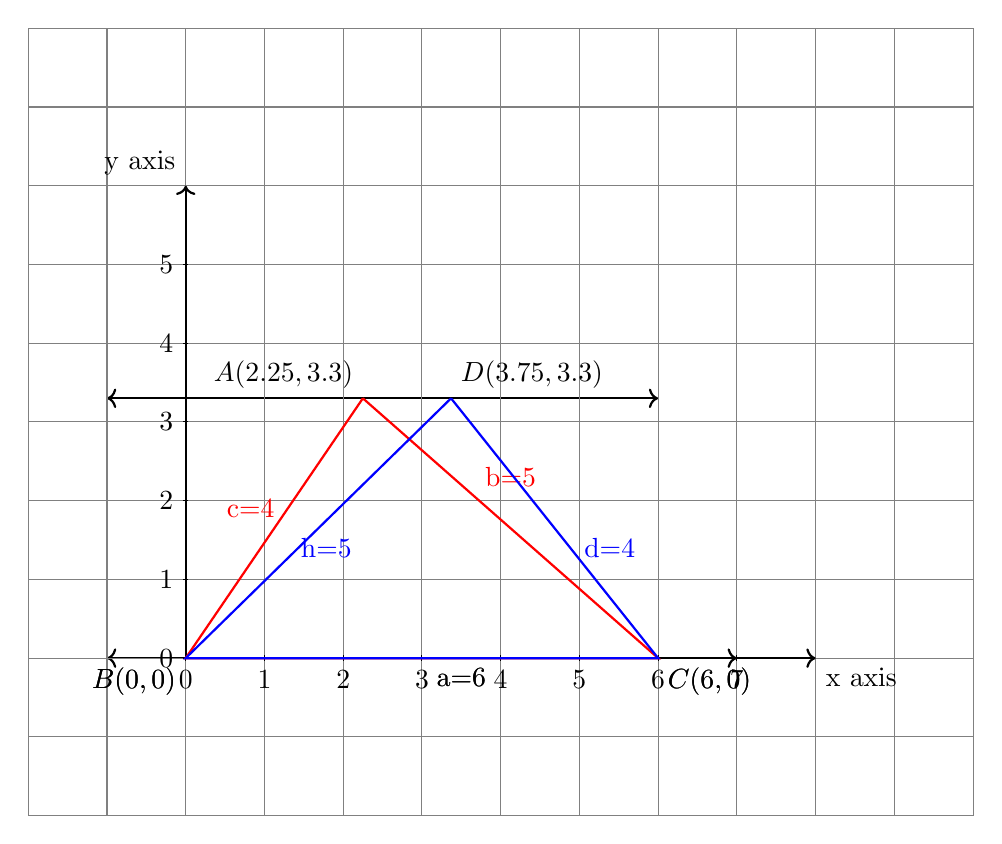
\begin{tikzpicture}

%genetrating parrallel lines
\draw[<->,black,thick] (-1,3.3)-- (6,3.3);
\draw[<->,black,thick] (-1,0)-- (7,0);

%generating grids
\draw[step=1cm,gray,thin] (-2,-2) grid(10,8);
\draw[thick,->] (0,0) -- (8,0) node[anchor= north west] {x axis};
\draw[thick,->] (0,0) -- (0,6) node[anchor = south east] {y axis};
\foreach \x in {0,1,2,3,4,5,6,7}
\draw (\x cm,1pt) -- (\x cm, -1pt) node[anchor=north] {$\x$};
\foreach \y in {0,1,2,3,4,5}
\draw (1pt,\y cm) -- (-1pt,\y cm) node[anchor= east] {$\y$};

% Defining the sides the Triangle ABC 
\def\a{6}
\def\b{5}
\def\c{4}
% sides of Triangle PBC
\def\a{6}
\def\d{4}
\def\h{5}

%Coordinates of A
\def\p{{\a^2+\c^2-\b^2}/{(2*\a)}}
\def\p{2.25}
\def\q{{sqrt(\c^2-\p^2)}}

%Labeling points of triangle ABC
\tkzDefPoint[label=above left:{$A(2.25,3.3)$}](2.25,3.3){A}
\tkzDefPoint[label=below left:{$B(0,0)$}](0,0){B}
\tkzDefPoint[label= below right:{$C(6,0)$}](6,0){C}

%Drawing triangle ABC
\draw[red,thick] (A) -- node[above,xshift=-3mm] {$\textrm{c=4}$} (B) -- node[black,below,xshift=5mm] {$\textrm{a=6}$} (C) -- node[above,yshift=4mm] {$\textrm{b=5}$} (A);

%Co-ordinates of D
\def\r{{\a^2+\h^2-\d'^2}/{(2*\a)}}
\def\r{3.75}
\def\s{{sqrt(\d'^2-\r^2)}}

%Labeling points of triangle DBC
\tkzDefPoint[label=above right:{$D(3.75,3.3)$}](3.37,3.3){D}
\tkzDefPoint[label=below left:{$B(0,0)$}](0,0){B}
\tkzDefPoint[label= below right:{$C(6,0)$}](6,0){C}

%Drawing triangle DBC
\draw[blue,thick] (D) -- node[below,xshift=1mm] {$\textrm{h=5}$} (B) -- node[black,below,xshift=5mm]{$\textrm{a=6}$} (C) -- node[below,xshift=7mm] {$\textrm{d=4}$} (D);
\end{tikzpicture}
\end{document}
